\documentclass[12pt]{article}
\usepackage[english]{babel}
\usepackage[utf8x]{inputenc}
\usepackage{amsmath}
\usepackage{graphicx}
\usepackage{subcaption}
\usepackage[colorinlistoftodos]{todonotes}
\usepackage{physics}
\usepackage{indentfirst}
\usepackage{appendix}
\usepackage{float}


\setlength{\marginparwidth}{2cm}
\begin{document}

\begin{titlepage}

\newcommand{\HRule}{\rule{\linewidth}{0.5mm}} % Defines a new command for the horizontal lines, change thickness here

\center % Center everything on the page
 

\textsc{\LARGE Aalto University}\\[1.5cm] % Name of your university/college

\includegraphics[scale=.1]{logo.png}\\[1cm] % Include a department/university logo - this will require the graphicx package
\textsc{\Large Methods of Data Mining}\\[0.5cm] % Major heading such as course name
\textsc{\large CS-E4650}\\[0.5cm] % Minor heading such as course title

\HRule \\[0.4cm]
{ \huge \bfseries Course Project}\\[0.4cm] % Title of your document
\HRule \\[1.0cm]

\begin{center}
José González López \\
893699\\
Cristian Manuel Abrante Dorta\\
888248
\end{center}

{\large \today}\\[2cm] 

\vfill % Fill the rest of the page with whitespace

\end{titlepage}

\setcounter{page}{1}
\tableofcontents

\newpage

\section{GeneData}

In this section the preprocesssing of data and results for the different clustering algorithms is presented, refer to the Appendix section in order to know more about the hypertuning (Section \ref{genedata:hypertuning}).

\subsection{Methods}

The first step for performing clustering was the data preprocessing. For this project, we followed a minimalist approach, applying simple techniques in the preprocessing at first, and then increasing the complexity of them if the clustering algorithms did not performed well. We had executed all the clustering algorithms with the different parameters combination using three different datasets:

\begin{itemize}
    \item \textbf{raw dataset}: In this case no preprocessing has been done to the dataset, only the class column has been removed.
    \item \textbf{Min max scaled dataset}: In this case, all data columns are scaled using \texttt{sklearn.preprocessing.MinMaxScaler}.
    \item \textbf{Standard scaled dataset}: All columns of the dataset are scaled using \texttt{sklearn.preprocessing.StandardScaler}.
\end{itemize}

\subsection{Results}

Here the results for each clustering algorithm are  presented. The quality of the results is based on the normalized mutual information (NMI) score. For the calculation of this index, the method \texttt{sklearn.metrics.normalized\_mutual\_info\_score} is used.

\begin{itemize}
    \item \textbf{K Means results}: For the different three preprocessed datasets and the different hyperparameters the results obtained are shown in Table \ref{res:k-means}. We can observe that the algorithm perform better where the data is not preprocessed, obtaining the best result for $k=6$ in the first execution, with an NMI of 0.88669.
    \item \textbf{Agglomerate hierarchical clustering results}: As in the previous section, the results for the three different datasets are shown in Table \ref{res:hier}. As in the previous case, the best results are obtained with no preprocessed data, using the ward linkage metric and 6 clusters, with an NMI of 0.92134.
    \item \textbf{Spectral clustering result}: Finally, the results for the spectral clustering algorithm are presented in Table \ref{res:spectal}. The best result was obtained with raw data again, achieving an NMI score of 0.98007 with nearest neighbors as affinity type, $k=5$ and $gamma = 1.5$.
\end{itemize}

\subsection{Conclusions}

After trying those three different clustering algorithms we can state that the best result is achieved with the spectral clustering, with an NMI superior to 0.98 using nearest neighbours as afinity type, $k=5$ and $gamma = 1.5$. It is surprising that the best score is obtained without preprocessing, and this could be due to the nature of data and possible due to the existence of underlying patterns, detected in the clustering algorithm, in the generation of it. \\

Future work can also be done with this dataset, especially if we take into consideration the possibility of adding new clustering algorithms that we can try, and also if we try more hyperparameters, possibly running the executions (which will be computationally demanding) in external services such as Google Cloud.

\section{MSData}
\subsection{Methods}
With this dataset, we decided to reduce the dimension of the columns as we had over 5000 features in total. As we did not have any information on what information was stored in each feature, each column was treated equally by first applying a Standard Scaler to uniform the data and reduce the possible noise and the possible impact of outliers. We did not detect any strange values nor missing values on the data so after that step we created a battery of clustering methods seen on class and execute them with different feature reduction provided by PCA. With exhaustive search for the best clustering method, it seemed that keeping 2 components was more than enough to get a NMI above 80\% in general (Section \ref{MSData:Table}). \\

Looking at the variance of the features, we could see that the columns in general (except the first one) carried the same variance/information, so this approach seemed quite justified, even if we were theoretically losing a lot of information in the process. There is not much sense in keeping low variance columns because we are not getting any information from them (individually speaking), losing information does not mean that we will have worse results and from the computation point of view, it is more efficient for the algorithms to work with simpler datasets.\\

To get a better look of the dataset we provide in the report the plot of the 2 principal components and the same plot but with the real labels (see appendix visualization of data). When we had a first look at the dataset, we thought that the clusters were rearranged quite differently but in the end, our best result was using 2 PCA components and spectral clustering with 6 clusters, $gamma=1.0$ (sklearn parameters) and a fully connected graph approach. (Section \ref{MSData:Vis}).\\

As for distance and similarity measures, in our trials we detected that in the transformed dataset the cosine distance was particularly effective in the Agglomerative clustering methods (Section \ref{MSData:Table}), but in the end, as we have stated before, the best results were achieved by using the rbf kernel (for constructing the similarity graph) of the spectral clustering algorithm.\\

\subsection{Results}
In the end we could separate the clusters almost perfectly on the left side, but the right side was predicted totally different than the real values. From our personal point of view, we could even  consider these group of points as outliers, still as we do not have any more information we cannot decide what to do with them on a real case scenario (Section \ref{MSData:Vis}). \\

In general our results may vary in the range of 88\%-85\% NMI score, but overall it has been pretty consistent over the runs (Section \ref{MSData:File}). 

\subsection{Conclusions}
After trying different methods and clustering algorithms, the best results were achieved by using PCA with two components in the standard scaled dataset with spectral clustering (6 clusters, $gamma=1.0$, rbf kernel). As we do not have enough information about the dataset (as it was artificially generated) and our validation measures justify our choice, we believe that we have managed to get a decent outcome. \\

We do not have any clear justification in why spectral clustering worked as well as why agglomerative clustering with cosine distance had much more better results than itself but with a different distance measures. We hypothesize that these results have to be bounded on how the points on the clusters are organized and reduced to 2 components.

\clearpage

\section{Appendix}
\appendix
%\appendixpage
%\addappheadtotoc
%\addcontentsline{toc}{chapter}{Apendix}

\section{Genedata}

In the appendix, it is explained how the preprocessing is done to data and the different hyperparameter combination done in order to choose the optimal values for the clustering algorithm.

\subsection{Clustering algorithms proposed}
\label{genedata:hypertuning}

For clustering the dataset, three different algorithms were proposed. Each of them was tuned separately using a certain combination of hyperparameters, in order to find the combination that gave as a result the highest NMI score.

\subsubsection{K Means clustering}

The first algorithm that was tested was k-means. The implementation available in \texttt{sklearn.cluster.KMeans} is the one used. The hyperparameter tuning in this case is not extend, because only two parameters has been tried:\\

\begin{itemize}
    \item \textbf{Number of clusters ($k$)}: number of clusters that the k-means algorithm is going to compute. For selecting the values, we have range between 2 and 10 clusters, based on the 5 possible values of classes presented in data.
    \item \textbf{Number of executions}: how many times the algorithm  will be executed for each number of cluster. This parameter is added for reduce the effect of randomness in the execution.
\end{itemize}

In table \ref{table:hyp-k-means} are stated the different possible values that we have for each parameter:

\begin{table}[h]
\centering
\begin{tabular}{l|l}
parameter              & possible values \\ \hline
number of clusters (k) & 2,3,4,5,6,10    \\
number of executions   & 5              
\end{tabular}
\caption{Hyperparameter values for $k$-means}
\label{table:hyp-k-means}
\end{table}

This combinations gave us 30 different executions for the algorithm.

\subsubsection{Agglomerate hierarchical clustering}

The second clustering algorithm tried was hierarchical algorithm clustering. In this case, the implementation used was the one of \texttt{scipy.cluster.hierarchy}. Two different parameters were tuned in this case:

\begin{itemize}
    \item \textbf{Linkage metric}:Is the method for the calculation of inter-cluster distances. The six available metrics in the external library were used.
    \item \textbf{Number of clusters}: Number of clusters that we are considering for computing the labels once the hierarchical clustering is computed.
\end{itemize}

The possible values for this parameters are shown in table \ref{table:hyp-hier}.

\begin{table}[h]
\centering
\begin{tabular}{l|l}
parameter            & possible values                                   \\ \hline
Linkage metric       & single, complete, average, centroid, median, ward \\
number of executions & 2,3,4,5,6,7                                      
\end{tabular}
\caption{Hyperparameter tuning for hierarchical agglomerative clustering}
\label{table:hyp-hier}
\end{table}

This parameters give us 36 possible combinations of executions.

\subsubsection{Spectral clustering}

The last clustering method tested was spectral clustering, using the execution available in \texttt{sklearn.cluster.SpectralClustering}. As it is a more complex algorithm, hyperparameter tuning was more complex, using three different parameters:

\begin{itemize}
    \item \textbf{Affinity type}: method used for constructing the affinity matrix.
    \item \textbf{Number of clusters}: In the same case as in previous methods, this is the number of clusters selected.
    \item \textbf{gamma}: this is the kernel coefficient used. It should be ignored when the affinity type is \textit{nearest neighbours}.
\end{itemize}

The possible combinations are expressed in the following table \ref{table:hyp-spectral}. \\

\begin{table}[H]
\centering
\begin{tabular}{ll}
\multicolumn{1}{l|}{parameter}          & possible values         \\ \hline
\multicolumn{1}{l|}{Affinity type}      & nearest\_neighbors, rbf \\
\multicolumn{1}{l|}{number of clusters} & 4,5,6                   \\
Gamma                                   & 0.5, 1.0, 1.5          
\end{tabular}
\caption{Hyperparameter tuning for hyerarchical clustering}
\label{table:hyp-spectral}
\end{table}

This combination of parameters gave us 18 different executions. Less combinations are tried in this case compared with the other algorithms because the computation time of the clustering algorithm is really extensive, and will take much more time if more combinations are tested.

\subsection{Results}

In this section are shown all the tables that are obtained with the different clustering algorithm.

\begin{table}[h]
\centering
\begin{tabular}{|cc|l|cc|l|cc|l|}
\hline
\multicolumn{3}{|c|}{No preprocessing}                            & \multicolumn{3}{c|}{Min Max Scaling}                             & \multicolumn{3}{c|}{Standard Scaling}                            \\ \hline
\multicolumn{1}{|l}{K} & \multicolumn{1}{l|}{Execution} & NMI     & \multicolumn{1}{l}{K} & \multicolumn{1}{l|}{Execution} & NMI     & \multicolumn{1}{l}{K} & \multicolumn{1}{l|}{Execution} & NMI     \\ \hline
6                      & 0                              & 0.88669 & 5                     & 4                              & 0.82783 & 5                     & 2                              & 0.79724 \\
6                      & 2                              & 0.88486 & 5                     & 0                              & 0.82599 & 5                     & 3                              & 0.79724 \\
6                      & 1                              & 0.88475 & 5                     & 3                              & 0.82215 & 5                     & 4                              & 0.79325 \\
6                      & 3                              & 0.88372 & 5                     & 2                              & 0.8207  & 5                     & 0                              & 0.78359 \\
6                      & 4                              & 0.88353 & 5                     & 1                              & 0.81881 & 10                    & 0                              & 0.78141 \\ \hline
\end{tabular}
\caption{Results of NMI for $k$ means algorithm}
\label{res:k-means}
\end{table}

\begin{table}[H]
\centering
\begin{tabular}{|cc|l|cc|l|cc|l|}
\hline
\multicolumn{3}{|c|}{No preprocessing}                          & \multicolumn{3}{c|}{Min Max Scaling}                           & \multicolumn{3}{c|}{Standard Scaling}                          \\ \hline
\multicolumn{1}{|l}{linkage} & \multicolumn{1}{l|}{K} & NMI     & \multicolumn{1}{l}{Linkage} & \multicolumn{1}{l|}{K} & NMI     & \multicolumn{1}{l}{Linkage} & \multicolumn{1}{l|}{K} & NMI     \\ \hline
ward                         & 6                      & 0.92134 & ward                        & 7                      & 0.86673 & ward                        & 7                      & 0.86682 \\
ward                         & 5                      & 0.88969 & ward                        & 6                      & 0.82745 & ward                        & 6                      & 0.83196 \\
ward                         & 7                      & 0.88449 & ward                        & 5                      & 0.81825 & ward                        & 5                      & 0.82946 \\
ward                         & 4                      & 0.82483 & ward                        & 4                      & 0.74042 & ward                        & 4                      & 0.75069 \\
ward                         & 3                      & 0.76123 & ward                        & 3                      & 0.67428 & ward                        & 3                      & 0.68164 \\ \hline
\end{tabular}
\caption{Results obtained for agglomerate hierarchical clustering}
\label{res:hier}
\end{table}

\begin{table}[h]
\centering
\begin{tabular}{|ccc|c|ccc|l|ccc|l|}
\hline
\multicolumn{4}{|c|}{No preprocessing} & \multicolumn{4}{c|}{Min Max Scaling}                 & \multicolumn{4}{c|}{Standard Scaling}                \\ \hline
Aff  & K  & Gamma  & NMI     & Aff & K & Gamma & \multicolumn{1}{c|}{NMI} & Aff & K & Gamma & \multicolumn{1}{c|}{NMI} \\ \hline
nn             & 5  & 1.5    & 0.98007 & nn            & 5 & 0.5   & 0.96127                  & nn            & 5 & 1.5   & 0.95138                  \\
nn             & 5  & 1.0    & 0.98007 & nn            & 5 & 1.5   & 0.96127                  & nn            & 5 & 1.0   & 0.95138                  \\
nn             & 5  & 0.5    & 0.98007 & nn            & 5 & 1.0   & 0.96127                  & nn            & 5 & 0.5   & 0.95138                  \\
nn             & 6  & 1.5    & 0.93436 & nn            & 6 & 1.5   & 0.87903                  & nn            & 6 & 1.5   & 0.89188                  \\
nn             & 6  & 1.0    & 0.93436 & nn            & 6 & 1.0   & 0.87903                  & nn            & 6 & 1.0   & 0.89188                  \\ \hline
\end{tabular}
\caption{Results obtained with spectral clustering}
\label{res:spectal}
\end{table}

Apart from that, three indices are calculated in order to test which are the optimal number of clusters using the best parameter configuration of the best result. Which is the spectral clustering with nearest neighbours affinity type and $gamma=1.0$. 

\begin{figure}[h]
    \centering
    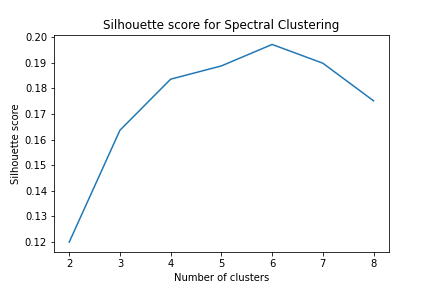
\includegraphics[scale=0.4]{best-ss.png}
\end{figure}

\begin{figure}[h]
    \centering
    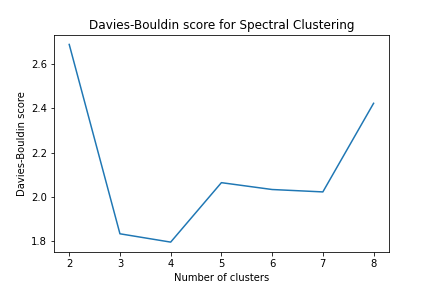
\includegraphics[scale=0.4]{best-db.png}
\end{figure}

\begin{figure}[H]
    \centering
    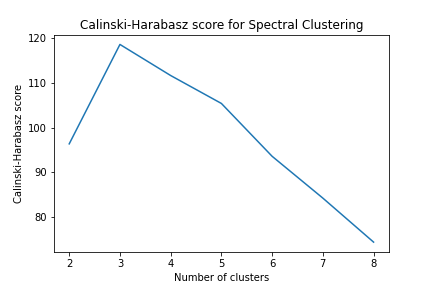
\includegraphics[scale=0.4]{best-ch.png}
\end{figure}

Having those indices, we can interpret that having the optimal number of clusters that we have calculated ($k=5$), is a good result according to both of the three indices. In silhouette score, even though it is not the best result, is one of the highest scores, which is still a good result. There is also a significant change when we observe Davies Bouldin score, because the score for $k=5$ is a higher than the best result which is $k=4$. Finally, taking into consideration the Calinski-Harabasz score, the number $k=5$ obtains an average higher, but still not be the best one, which is $k=3$.\\

Even though for this project the chosen goodness measure is NMI, we can also justify that good results are obtained with those three additional metrics.

\section{MSData}
\subsection{How to run the files} \label{MSData:File}
For the MSData, we provide 2 python files, one called battery-msdata- pca.py which contains multiple test done with different algorithms and it was used to get an overview of what was the best way to reduce the data set and also compare which solutions worked better. This program can be customize in terms of choosing whit algorithms to run by changing the value of the boolean variables at the beginning of the main function. \\

\textbf{Note}: Running all test will result in a long run (about 3-4 minutes). \\

The other file is called msdata.py, which is the main program that computes the best algorithms with the best parameters possible (mainly obtained by the other program and some individual trials for the spectral clustering) and in the end it will use spectral clustering on the transformed data set to create a txt file. this file will contain in the i th row the value of the cluster assigned to the i th point. There are two boolean variables, \textit{ignore} will show the plots of the data set, and the calculation of the validation metrics of each algorithm to get the optimal number of clusters for each case. \textit{Test} will enable the creation of such algorithms so that in the end it will print the from best to worst (with their optimal number of clusters according to metrics). Enabling this option should return spectral clustering on first place on the final list, meaning that is the most suited one and hence our solution algorithm (see appendix justification for more info). \\ 

\textbf{Final note}: To run the files
\begin{itemize}
    \item Use python 3.5.3 or above
    \item The csv file should be in the same directory as the py file.
    \item Some libraries such as sklearn, pandas, numpy, matplotlib, collections and scipy are required.
\end{itemize} 

\subsection{Visualization of the data}\label{MSData:Vis}
The following pictures show some visualizations used for the ms data set.

\begin{figure}[H]
     \centering
     \begin{subfigure}[b]{0.4\textwidth}
         \centering
         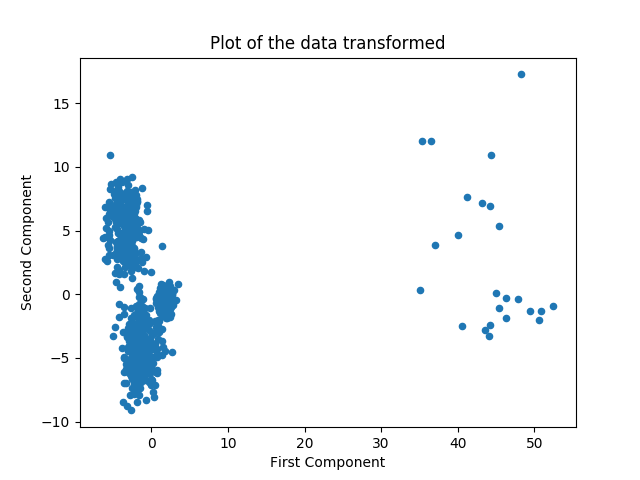
\includegraphics[width=\textwidth]{Figure_1.png}
         \caption{Data with 2 components}
     \end{subfigure}
     \hfill
     \begin{subfigure}[b]{0.4\textwidth}
         \centering
         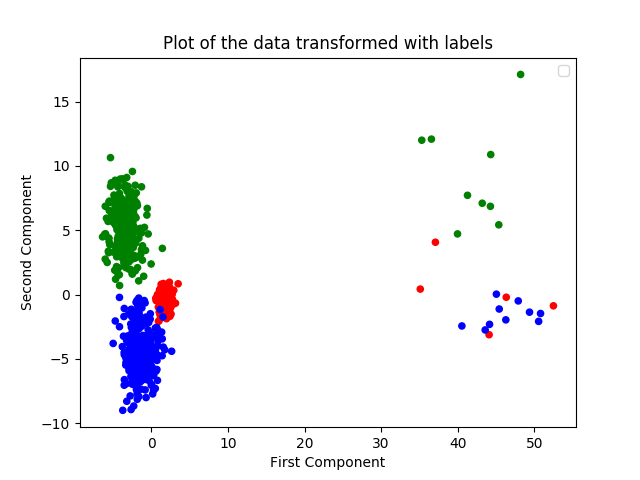
\includegraphics[width=\textwidth]{Figure_26.png}
         \caption{Data with real labels}
     \end{subfigure}
\end{figure}

\begin{figure}[H]
    \centering
    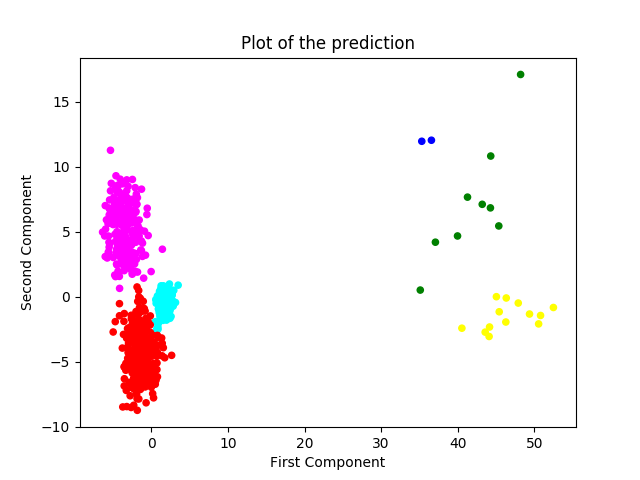
\includegraphics[scale=0.5]{Figure_27.png}
    \caption{Our prediction}
\end{figure}

\subsection{Table of NMI scores}\label{MSData:Table}
Here we show the top 10 algorithms that we tested in our battery program and in individual trials.\\

\resizebox{13cm}{!}{
\begin{center}
 \begin{tabular}{||c c c c c c||} 
 \hline
 Algorithm & N Clusters & Linkage & Affinity & PCA components & NMI score \\ [0.5ex] 
 \hline\hline
 Spectral & 6 & - & - & 2 & 0.8705695304627331\\
 \hline
 Agglomerative  & 3 & Complete & Cosine & 2 & 0.8704595404687339\\
 \hline
 Agglomerative  & 6 & Single & Cosine & 2 & 0.8527480849011208\\
 \hline 
 Agglomerative  & 3 & Average & Cosine & 4 & 0.8308527272121102\\
 \hline
 Agglomerative  & 7 & Single & Cosine & 2 & 0.8276498843162884\\
 \hline
 Agglomerative  & 3 & Average & Cosine & 2 & 0.8187407994276206\\
 \hline 
 Agglomerative  & 4 & Average & Cosine & 2 & 0.8151717946668879\\ 
 \hline
 Agglomerative  & 4 & Complete & Cosine & 2 & 0.7909766331843715\\ 
 \hline
 Agglomerative  & 5 & Average & Cosine & 2 & 0.7860058411489088 \\[1ex] 
 \hline
\end{tabular}

\end{center}
}

\subsection{Justification of chosen algorithm and parameters} \label{MSData:Jus}
Applying some metrics such as Silhouette, Calinski-Harabasz and  Davies-Bouldin scores we could get the optimal number of clusters for the best algorithms we got from the battery of algorithms. For example, for our solution

\begin{figure}[H]
    \centering
    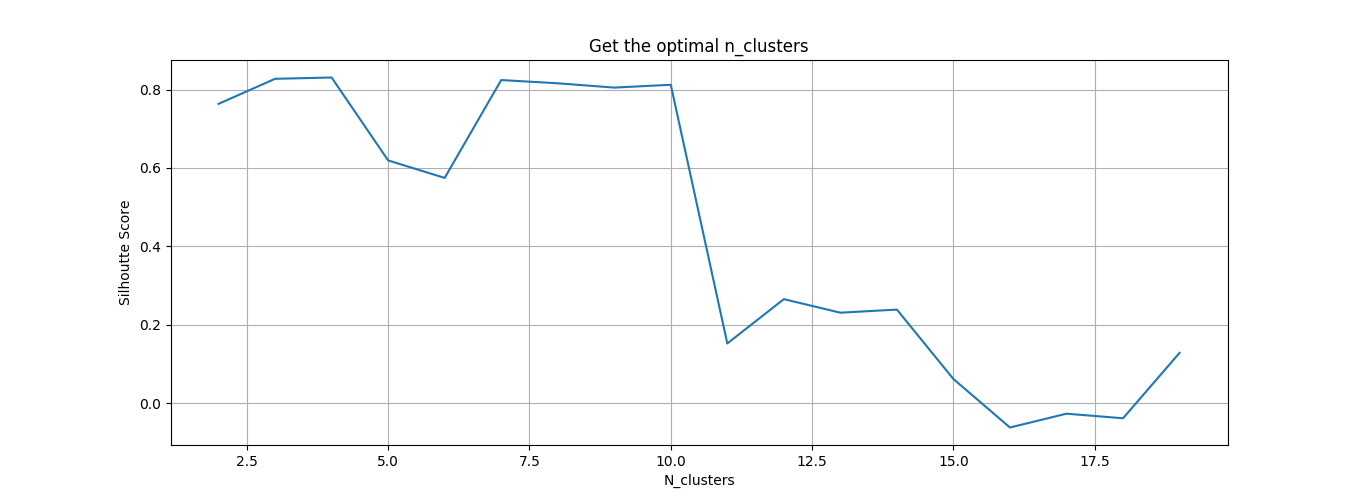
\includegraphics[scale=0.4]{Figure_17(SpecClus_10_Silhouette).png}
    \caption{Silhouette score}
\end{figure}

\begin{figure}[H]
    \centering
    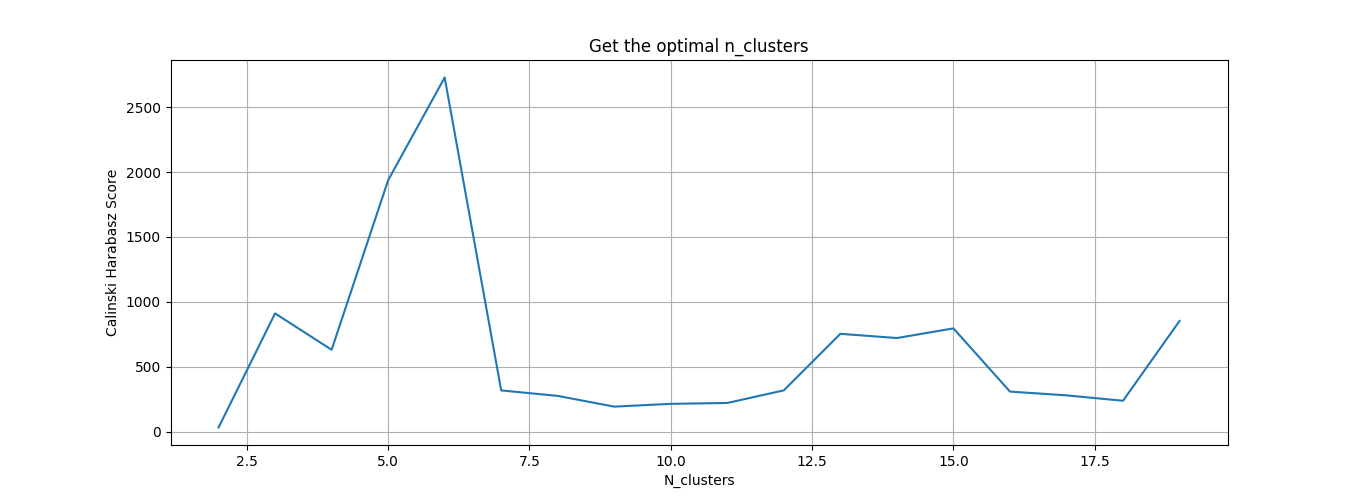
\includegraphics[scale=0.4]{Figure_18(SpecClus_10_Calinski).png}
    \caption{Calinski-Harabasz score}
\end{figure}

\begin{figure}[H]
    \centering
    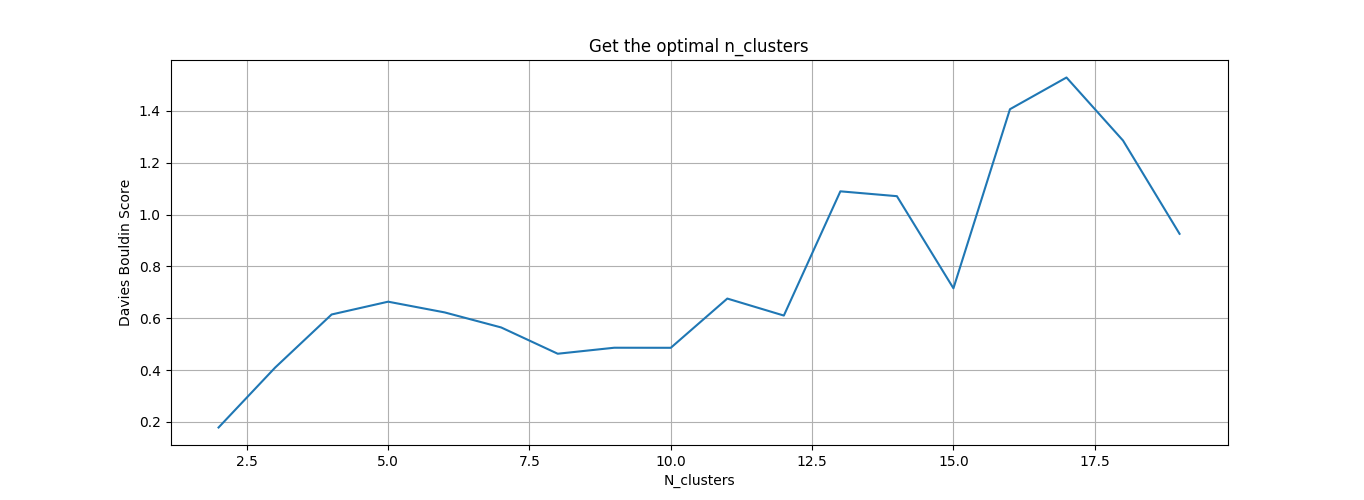
\includegraphics[scale=0.4]{Figure_19(SpecClus_10_Davies).png}
    \caption{Davies-Bouldin score}
\end{figure}

in this case, the Silhouette score is high with 3 or 7 clusters (not 6), but it reaches a high peak in the Calinski-Score with 6 clusters and it maintains a low level in the Davies Bouldin study, so that's the reason we chose 6 clusters. \\

We have generated the same plots for each algorithm, but for the sake of making this report as concise as possible we did not include them here.
\end{document}
